\documentclass[a4paper,oneside]{article}
\usepackage{geometry}
\usepackage[latin1]{inputenc}
\usepackage[catalan]{babel}
\usepackage{amsfonts}
\usepackage{graphicx}
\usepackage{fancyvrb}
\usepackage{listings}
\usepackage{url} 

\usepackage[pdfauthor={Ramon Xuriguera Albareda},%
		pdfsubject={BibTeX Bibliography Index Maker},%
		pdftitle={BibTeX Bibliography Index Maker: Notes},%
		pdftex]{hyperref}

\lstset{numbers=left,breaklines=true,fancyvrb=false}		

\title{BibTeX Bibliography Index Maker: Notes}
\author{Ramon Xuriguera}
\date{}

\begin{document}
\maketitle

\section{BibTeX}
Aspectes del format BibTeX a tenir en compte:
\begin{itemize}
\item{Com podem distingir entre diferents tipus d'entrada (article, book, inproceedings, etc.) a partir del fitxer?}
\item{Format dels noms. Un nom consisteix de diferents parts: First, von, Last, Jr. El token \textit{von} o \textit{de la} cal posar-los
en min�scules. Per tal que el nom es reconegui, cal que tingui el format: von Last, Jr, First. D'aquesta manera, si hi ha m�s d'un
cognom no passa res.}
\item{Car�cters Unicode entre claus per poder ser utilitzats correctament amb l'estil \textit{alpha}. Per exemple: \verb=Jos{\'{e}}=}
\item{Per prevenir que BibTeX canvi� un text a min�scules, cal posar el text entre claus.}
\item{Si hi ha massa autors, truncar la llista amb \textit{et al.}}
\item{Utilitzar abreviatures de tres lletres per als mesos}
\item{Utilitzar el camp \texttt{key} per a organitzacions amb un nom llarg, de manera que s'utilitzin les inicials de l'organitzaci� 
al fer una cita.}

\end{itemize}

\section{Extracci� del contingut dels fitxers PDF}
Aspectes a considerar:
\begin{itemize}
\item{Car�cters Unicode}
\item{Glyphs com ara \textit{fi} corresponen a m�s d'una lletra}
\item{Les llibreries extreuen el text per l�nies}
\item{Podem obtenir les seg�ents dades del fitxer sense
haver-ne d'extreure el text: n�mero de p�gines, t�tol, autor, assumpte i paraules clau. Si aquests camps no s'han omplert al 
generar el fitxer, estaran en blanc.}
\end{itemize}

\subsection{Software}
\begin{itemize}
\item{xPDF}
Proporciona eines executables des de la l�nia de comandes per extreure el text.
Nom�s converteix a text pla, per� no separa els diferents par�grafs en l�nies diferents. Permet obtenir el resultat en diferents
codificacions de car�cters, per� no conserva els text correcte. �s a dir, continua tenint problemes per extreure accents, etc.
Amb l'eina \texttt{pdftohtml} podem obtenir informaci� d'algunes de les paraules en negreta, per� separa cada l�nia amb una etiqueta
br.
\item{PDFBox}
Llibreria escrita en Java i publicada sota la llic�ncia \textit{Apache License v2.0}. Actualment es troba a la incubadora d'Apache. 
Permet obtenir el text i les metadades d'un fitxer. Separa els resultats per l�nia segons es troben en el document, no per par�grafs.
\end{itemize}



\subsection{Procediment}


\section{Articles Db}
\begin{description}
\item{\textbf{Google Scholar/Google Search API}}\\
Enlla� directe a la cita en format BibTeX. Actualment no proporcionen cap API per obtenir-ho. Caldria fer-ho amb \texttt{wget}.
\item{\textbf{DBLP}}\\
DBLP proporciona una API molt simple per cercar autors autors i obtenir les seves publicacions, per� no al rev�s. Al cercar per autor, es mostren
les claus de cada publicaci�, per� no el t�tol.
\item{\textbf{Portal ACM}}
\item{\textbf{CiteSeerX}}
\item{\textbf{Arxiv.org}}\\
	\url{http://arxiv.org/help/api/index}
\end{description}

\section{JabRef}
Java, llic�ncia: LGPL.
\\
�s possible crear plug-ins amb \textit{Java Plug-in Framework}. L'�ltima versi� d'aquest framework �s de fa m�s de dos anys, actualment es troba en
estat \textit{frozen} i �s pre-OSGi. En el f�rum i el tracker de \textit{JabRef} no hi ha cap missatge en el que es discuteixin canvis sobre aquest tema. \\
Extension-points permesos:
\begin{itemize}
\item{\textbf{ImportFormat}} 
Add importers to JabRef accessible from the 'Import into ... database'.
\item{EntryFetcher}
Add access to databases like Citeseer or Medline to the Web Search menu.
\item{ExportFormatTemplate}
Add a template based export like the ones accessible using the Manage Custom Exports.
\item{ExportFormat}
Add an export filter to JabRef's export dialog, that is more complicated than the simple template based one.
\item{ExportFormatProvider}
A more powerful way to add export formats to JabRef.
\item{LayoutFormatter}
Add formatters that can be used in the layout based exporters.
\item{\textbf{SidePanePlugin}}
Add a side pane component that can do any kinds of operations. The panel is accessed from a Plugins menu in JabRef's main window.
\end{itemize}

\section{Llenguatge}
La idea seria desenvolupar una aplicaci� de l�nia de comandes amb \textit{Jython}, Python sobre la JVM i utilitzar 

\appendix
\section{Exemples de text extret}
A continuaci� es mostren algunes cap�aleres d'articles i el resultat obtingut a l'extreure'n el text:
\begin{itemize}

\item{Text 1}
    PDF:
    \begin{figure}[h]
    \begin{center}
    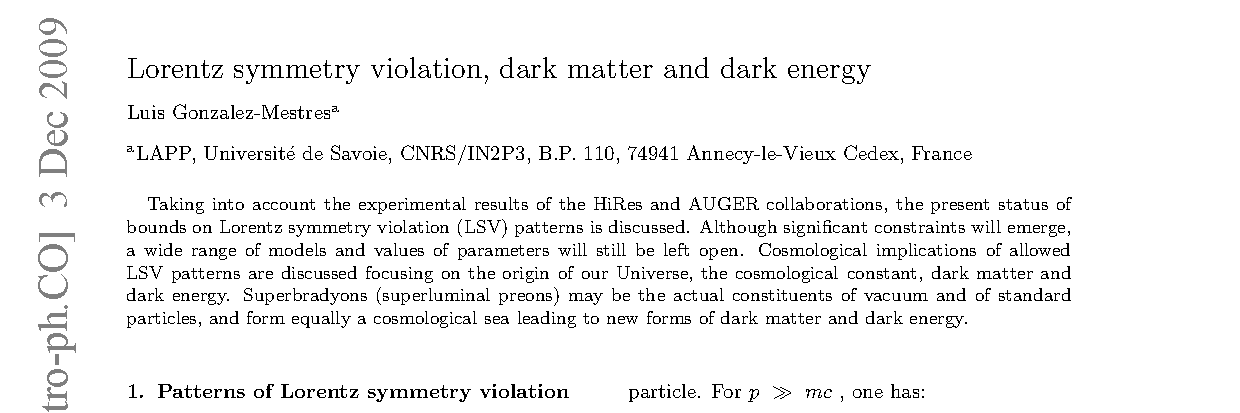
\includegraphics[scale=0.7]{images/article01Header.pdf}
    \end{center}
    \end{figure}
    
    Text pla:
    \begin{minipage}{0.8\textwidth}
    \begin{Verbatim}
    arXiv:0912.0725v1 [astro-ph.CO] 3 Dec 2009

    Lorentz symmetry violation, dark matter and dark energy
    Luis Gonzalez-Mestresa
    a

    LAPP, Universit de Savoie, CNRS/IN2P3, B.P. 110, 74941 Annecy-le-Vieux Cedex, France e

    Taking into account the experimental results of the HiRes and AUGER collaborations, the present status of bounds on Lorentz symmetry violation (LSV) patterns is discussed. Although significant constraints will emerge, a wide range of models and values of parameters will still be left open. Cosmological implications of allowed LSV patterns are discussed focusing on the origin of our Universe, the cosmological constant, dark matter and dark energy. Superbradyons (superluminal preons) may be the actual constituents of vacuum and of standard particles, and form equally a cosmological sea leading to new forms of dark matter and dark energy.

    1. Patterns of Lorentz symmetry violation A formulation of Planck-scale Lorentz symmetry violation (LSV) testable in ultra-high energy cosmic-ray (UHECR) 
    \end{Verbatim}
    \end{minipage}
    
    HTML:
    \begin{minipage}{0.8\textwidth}
    \begin{Verbatim}    
    <!DOCTYPE HTML PUBLIC "-//W3C//DTD HTML 4.01 Transitional//EN"><HTML>
    <HEAD>
    <TITLE></TITLE>
    </HEAD>
    <BODY>
    <A name=1></a>Lorentz symmetry violation, dark matter and dark energy<br>
    Luis Gonzalez-Mestresa<br>
    aLAPP, Universite de Savoie, CNRS/IN2P3, B.P. 110, 74941 Annecy-le-Vieux Cedex, France<br>
    Taking into account the experimental results of the HiRes and AUGER collaborations, the present status of<br>
    bounds on Lorentz symmetry violation (LSV) patterns is discussed. Although significant constraints will emerge,<br>a wide range of models and values of parameters will still be left open. Cosmological implications of allowed<br>LSV patterns are discussed focusing on the origin of our Universe, the cosmological constant, dark matter and<br>dark energy. Superbradyons (superluminal preons) may be the actual constituents of vacuum and of standard<br>particles, and form equally a cosmological sea leading to new forms of dark matter and dark energy.<br>
    1. Patterns of Lorentz symmetry violation<br>
    \end{Verbatim}
    \end{minipage}
\item{Text 2}    
\end{itemize}

\end{document}